\documentclass[
    ngerman,
    accentcolor=3b,
    % dark_mode, % uncomment for dark mode
    fontsize= 12pt,
    a4paper,
    aspectratio=169,
    colorback=true,
    fancy_row_colors,
    leqno,
    fleqn,
    boxarc=3pt,
    fleqn,
    main,
    % shell_escape = false, % Kompatibilität mit sharelatex
]{algoslides}

%%------------%%
%%--Packages--%%
%%------------%%

% \usepackage{audutils}
% \usepackage{fopbot}
\usepackage{booktabs}
\usepackage{tipa}


%%----------------------------%%
%%--Stilistische Anpassungen--%%
%%----------------------------%%


\renewcommand\tabularxcolumn[1]{m{#1}}% for vertical centering text in X column
% Remove unwanted space from tables
\aboverulesep = 0mm \belowrulesep = 0mm
\renewcommand{\arraystretch}{1.4}

%%---------------------------%%
%%--Dokumenteneinstellungen--%%
%%---------------------------%%

% Workshop-Individuelle Einstellungen
\def\workshoptitle{\LaTeX}
\def\shortworkshoptitle{\LaTeX}
\subtitle{Einsteiger Workshop}
\def\gruesswoerte{Gude}
\author{Ruben Deisenroth}
\titlegraphic*{\includegraphics{LaTeX-Wallpaper.png}}


% Ophase-Einstellungen
\ExplSyntaxOn
\def\summerophasename{Sommerophase}
\def\winterophasename{Winterophase}
\DeclareDocumentCommand{\ophase}{}{
    \int_compare:nTF {\the\month > 4}{
        \winterophasename\space{}\the\year-\the\numexpr\year+1\relax
    }{
        \summerophasename\space{}\the\year
    }
}
\ExplSyntaxOff
\graphicspath{{pictures}}
\title[\shortworkshoptitle{}]{\workshoptitle{}}
\department{TU Darmstadt | Fachbereich Informatik | \ophase{} | \insertshorttitle{}}
\date{\today}
\logo*{
\includegraphics{d120-logo.png}}
\def\codeDir{code}

%%-------------------------%%
%%--Beginn des Dokumentes--%%
%%-------------------------%%

\begin{document}

    %%-----------%%
    %%--Titelei--%%
    %%-----------%%

    \maketitle{}

    \begin{frame}[c]
        % Die Begrüßenden Worte können individuell pro Workshop festgelegt werden. Am Besten nur was kurzes, sowie "Gude", "Hi", "Herzlich Willkommen!", ...
        \centering\huge\textbf{\gruesswoerte{}}
    \end{frame}

    %%---------------------------%%
    %%--Beginn der Präsentation--%%
    %%---------------------------%%

    \begin{frame}
        \frametitle{Das steht heute auf dem Plan}
        \tableofcontents[subsubsectionstyle=hide]
    \end{frame}


    %%-----------%%
    %%--Kapitel--%%
    %%-----------%%

    % !TeX root = ../main.tex
\documentclass[
    ngerman,
    accentcolor=3b,
    dark_mode,
    fontsize= 12pt,
    a4paper,
    aspectratio=169,
    colorback=true,
    fancy_row_colors,
    leqno,
    fleqn,
    boxarc=3pt,
    fleqn,
    design=2008,
    % shell_escape = false, % Kompatibilität mit sharelatex
]{algoslides}

%%--------------------------%%
%%--Imports from Main File--%%
%%--------------------------%%
\usepackage{import}
% Import all Packages from Main Preamble with relative Path (buggy, list packages instead)
\subimport*{../shared}{preamble}
% Get Labels from Main Document using the xr-hyper Package
\externaldocument[ext:]{../main}
% Set Graphics Path, so pictures load correctly
\graphicspath{{../pictures}}
\def\codeDir{../code}

\begin{document}
    \section{Einführung}\label{1}\label{Einfuehrung}
    \subsection{Was ist \LaTeX?}\label{1.1}\label{1.1}
    \begin{frame}[c]
        \slidehead{}
        \centering\fontsize{40pt}{45pt}\selectfont\LaTeX

        %ˈlaːtɛç
        \medskip\normalsize\textipa{[\textprimstress{}latE\c{c}]}

        \vfill
        LaTeX ist eine Programmiersprache zur Erstellung von PDF-Dokumenten. Erstveröffentlichung 1984
    \end{frame}
    \subsection{Idee von \LaTeX}\label{1.2}\label{1.2}
    \begin{frame}
        \slidehead{}
        \begin{itemize}
            \item Der \LaTeX-Quellcode wird zu PDF (oder SVG) kompiliert
            \item Trennung von Inhalt und Design
            \item Häufig verwendeten Code in wiederverwendbaren Commands zusammenfassen
            \item Man erhält \fatsf{exakt} das, was man hinschreibt
        \end{itemize}
    \end{frame}
    \subsection{Anwendungsmöglichkeiten}
    \begin{frame}
        \slidehead{}
        \begin{itemize}
            \item Arbeiten (z.B. Thesis)
            \item Hausübungsabgaben
            \item Zusammenfassungen
            \item Präsentationen (wie diese)
            \item Handouts
            \item Wissenschaftliches Zeichnen (z.B. Schaltplan, Diagramme, Moleküle, $\dots$)
            \item Vektorgrafiken
            \item Musik komponieren
            \item $\dots$
        \end{itemize}
    \end{frame}
\end{document}

    \documentclass[
    ngerman,
    accentcolor=3b,
    dark_mode,
    fontsize= 12pt,
    a4paper,
    aspectratio=169,
    colorback=true,
    fancy_row_colors,
    leqno,
    fleqn,
    boxarc=3pt,
    fleqn,
    % shell_escape = false, % Kompatibilität mit sharelatex
]{algoslides}

%%--------------------------%%
%%--Imports from Main File--%%
%%--------------------------%%
\usepackage{import}
% Import all Packages from Main Preamble with relative Path (buggy, list packages instead)
\subimport*{../shared}{preamble}
% Get Labels from Main Document using the xr-hyper Package
\externaldocument[ext:]{../main}
% Set Graphics Path, so pictures load correctly
\graphicspath{{../pictures}}
\def\codeDir{../code}

\begin{document}
    \section{Vor- und Nachteile von \LaTeX}\label{2}\label{2}
    \subsection{Vorteile}\label{2.1}\label{2.1}
    \begin{frame}
        \slidehead{}
        \begin{itemize}
            \item Einfache (nachträgliche) Änderung des Design
            \item Automatisierung
                \begin{itemize}
                    \item Seitennummer,
                    \item Inhaltsverzeichnis,
                    \item Abbildungsverzeichnis,
                    \item Literaturverzeichnis,
                \end{itemize}
            \item Fußnoten, Referenzen, Formatierung, $\dots$ sind einfach zu managen
            \item Formeln zu tippen ist intuitiv und einfach
            \item Stabil auch bei sehr großen Dokumenten
            \item Plattformunabhängig\begin{itemize}
                    \item Linux: TeXLive
                    \item Windows: TexLive oder MikTex
                    \item MacOS: TeXLive
                \end{itemize}
            \item Viele nützliche Pakete, die einem das Leben einfach machen
        \end{itemize}
    \end{frame}
    \begin{frame}[c]
        \begin{figure}[ht!]
            \centering
            \colorbox{white}{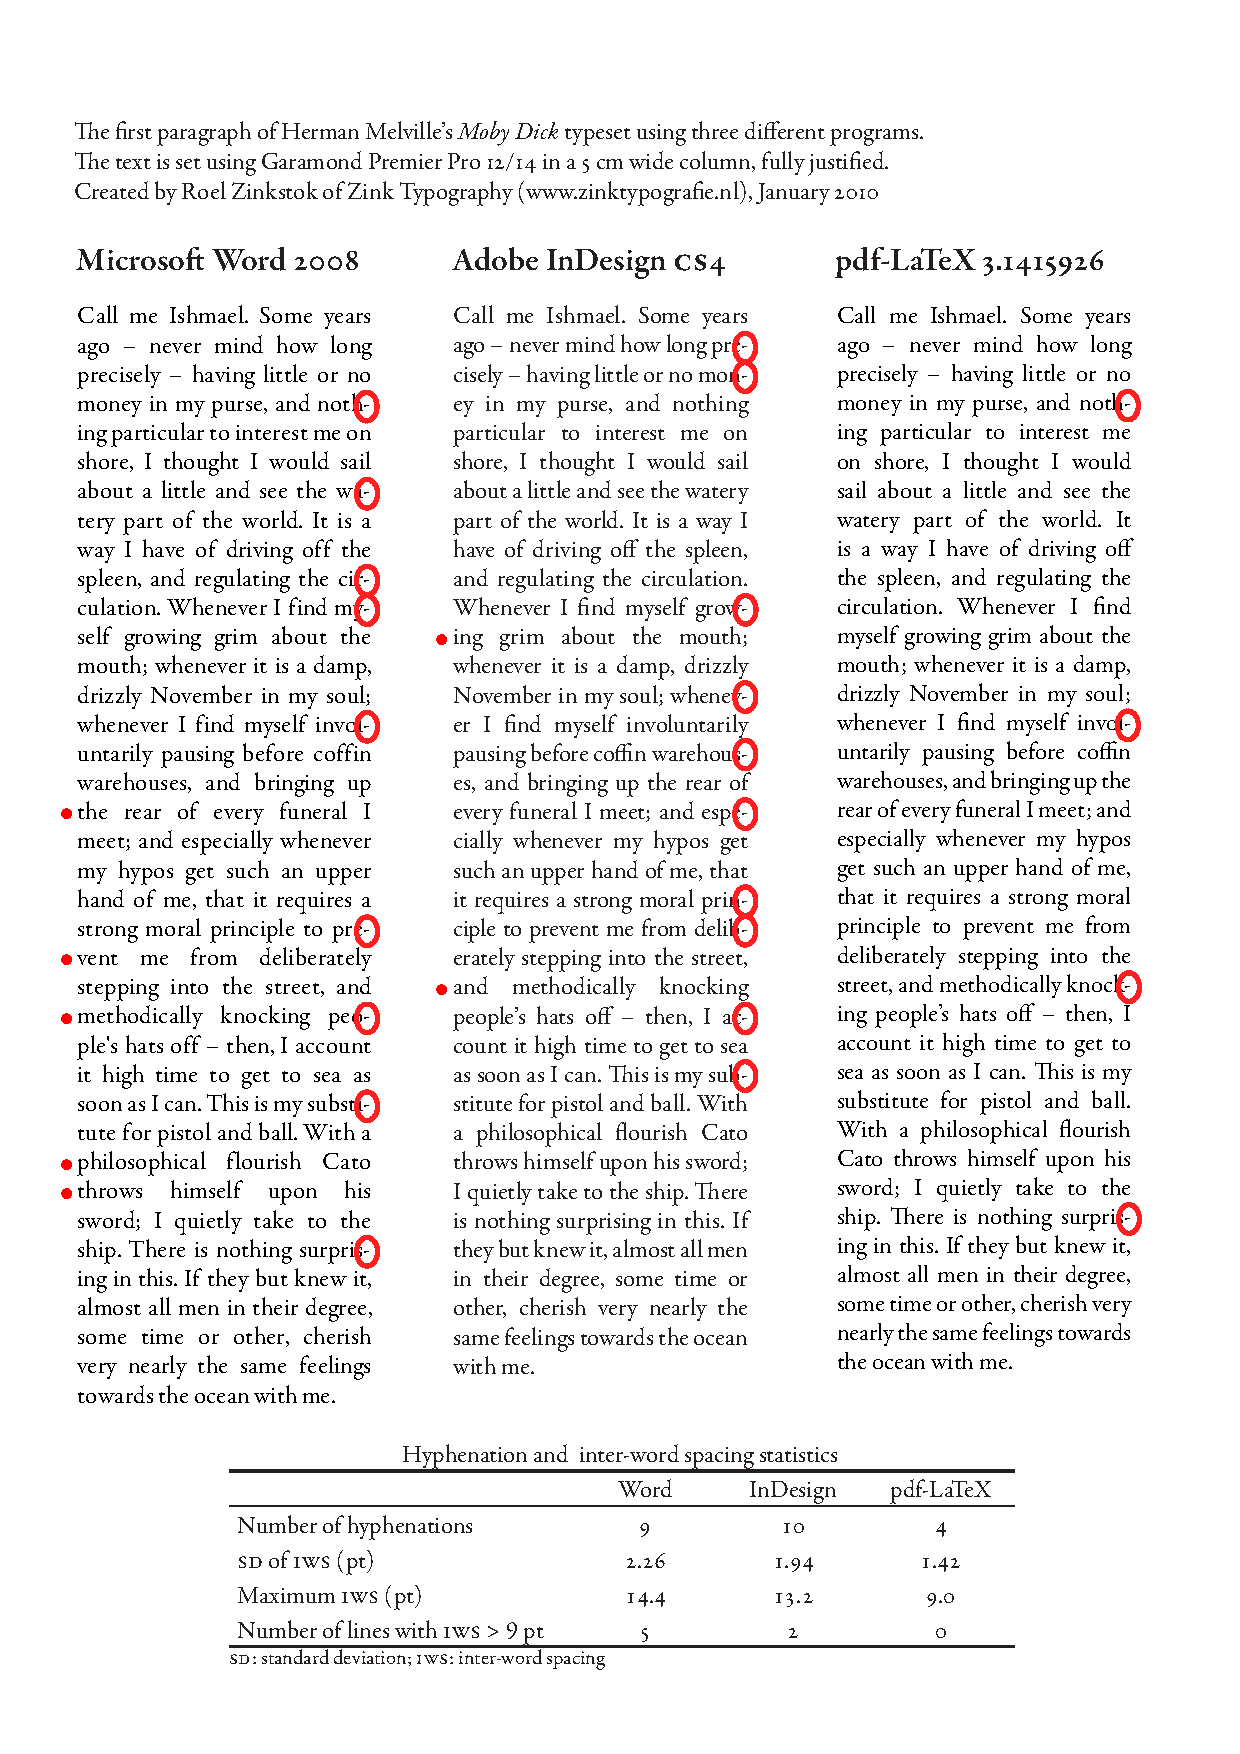
\includegraphics[height=6.5cm]{LaTeX vs Word vs Indesign.pdf}}
            \caption{Vergleich von \LaTeX, Word und InDesign}
            \label{fig:LaTeX-Vergleich}
        \end{figure}
    \end{frame}
    \subsection{Nachteile}\label{2.2}\label{2.2}
    \begin{frame}
        \slidehead{}
        \begin{itemize}
            \item Ungewohnt (auch wenn man schon einige Programmier- und Markup Sprachen kennt)
            \item Kein WYSIWYG (What you see is what you get)
                \begin{itemize}
                    \item Bis man Änderungen sieht kann lange dauern (gerade bei großen Dokumenten)
                \end{itemize}
            \item Steile Lernkurve
            \item Mehr Text, um Dinge zu beschreiben
        \end{itemize}
    \end{frame}
    \subsection{Komplexität}\label{2.3}\label{2.3}
    \begin{frame}
        \slidehead{}
        \tikzset{
            mylegend/.style={
                fgcolor,
                fill=\IfDarkModeTF{.!20!\thepagecolor}{.!20!\thepagecolor},
                fill opacity=0.9,
                draw=none,
                draw opacity=1,
                text opacity=1,
                rounded corners=3pt,
            },
        }
        \begin{figure}[ht!]
            \centering
            \begin{tikzpicture}
                \begin{axis}[
                        axis lines=center,
                        width=12cm,height=6cm,
                        xmin=0,
                        xmax=10,
                        ymin=0,
                        ymax=4,
                        xlabel={Aufwand},
                        ylabel={Komplexität des Dokuments},
                        legend style={
                            mylegend,
                            % at={(0.18,0.71)},
                            % anchor=north west
                        },
                        ticks=none,
                    ]
                    \addplot[samples=100,smooth, teal,thick] coordinates {
                        (0,0.4)
                        (.5,2)
                        (2,2.3)
                        (5,2.5)
                        (10,2.8)
                    };
                    \addlegendentry{Word};
                    \addplot[samples=100,smooth, orange,thick] coordinates {
                        (0,0.2)
                        (2,.5)
                        (4,2.5)
                        (8,8.6)
                    };
                    \addlegendentry{\LaTeX};
                \end{axis}
            \end{tikzpicture}
            \caption{Dokumentenkomplexität \LaTeX vs Word}%
            \label{fig:latex_vs_word}
        \end{figure}
    \end{frame}
\end{document}

    % !TeX root = ../main.tex
\documentclass[
    ngerman,
    accentcolor=3b,
    dark_mode,
    fontsize= 12pt,
    a4paper,
    aspectratio=169,
    colorback=true,
    fancy_row_colors,
    leqno,
    fleqn,
    boxarc=3pt,
    fleqn,
    % shell_escape = false, % Kompatibilität mit sharelatex
]{algoslides}

%%--------------------------%%
%%--Imports from Main File--%%
%%--------------------------%%
\usepackage{import}
% Import all Packages from Main Preamble with relative Path (buggy, list packages instead)
\subimport*{../shared}{preamble}
% Get Labels from Main Document using the xr-hyper Package
\externaldocument[ext:]{../main}
% Set Graphics Path, so pictures load correctly
\graphicspath{{../pictures}}
\def\codeDir{../code}

\begin{document}
    \section{\LaTeX-Basics}\label{2}\label{LaTeX-Basics}
    \subsection{Syntax}
    \begin{frame}[fragile]
        \slidehead{}
        \begin{itemize}
            \item Zeichen mit besonderer Bedeutung: \verb+\+, \verb+&+, \verb+#+, \verb+$+, \verb+%+, \verb+~+, \verb+^+, \verb+_+, \verb+{+, \verb+}+, \verb+[+ und \verb+]+
            \item Kommandos beginnen mit einem Backslask: \verb+\+
            \item Kommandonamen enthalten keine Zahlen, Leerzeichen und Sonderzeichen
            \item Argumente werden in geschweiften Klammern angegeben \verb+{}+
            \item Optionale Argumente werden in eckigen Klammern angegeben \verb+[]+
            \item Environments werden mit \verb+\begin{<name>}+ und \verb+\end{<name>}+ angegeben
            \item Kommentare beginnen mit einem \verb+%+
            \item Parameter werden mit \verb+#+ angegeben und gehen von 1-9\begin{itemize}
                    \item Dabei wird für innere Argumente die Anzahl der \verb+#+ verdoppelt (z.B. \verb+#1+, \verb+##1+, \verb+####1+)
                \end{itemize}
        \end{itemize}
    \end{frame}
    \subsection{Aufbau eines Dokumentes}\label{2.1}\label{2.1}
    \begin{frame}[fragile]
        \slidehead{}
        \begin{columns}[c]
            \begin{column}{.5\textwidth}
                \inputCode[]{
                    minted language=latex,
                    title=\codeBlockTitle{Minimales \LaTeX-Dokument},
                }{\codeDir/minimal.tex}
            \end{column}%
            \begin{column}{.5\textwidth}
                \centering
                \colorbox{white}{%
                    \color{black}
                    \includegraphics[width=\textwidth,height=5cm,keepaspectratio]{\codeDir/minimal}
                }
            \end{column}
        \end{columns}
    \end{frame}
    \subsubsection{Dokumentenklasse}
    \begin{frame}[fragile]
        \slidehead{}
        \begin{columns}[c]
            \begin{column}{.5\textwidth}
                \inputCode[highlightlines={1}]{
                    minted language=latex,
                    title=\codeBlockTitle{Minimales \LaTeX-Dokument},
                }{\codeDir/minimal.tex}
            \end{column}%
            \begin{column}{.5\textwidth}
                \centering
                \colorbox{white}{%
                    \color{black}
                    \includegraphics[width=\textwidth,height=5cm,keepaspectratio]{\codeDir/minimal}
                }
            \end{column}
        \end{columns}
    \end{frame}

    \begin{frame}[c,fragile]
        \slidehead{}
        Häufig verwendete Dokumentenklassen:
        \begin{itemize}
            \item \verb+article+ (Standardklasse für allgemeine Dokumente)
            \item \verb+book+ (Bücher)
            \item \verb+beamer+ (Präsentationen)
            \item \verb+standalone+ (Allenstehende Abbildungen)
        \end{itemize}
        \pause{}
        Klassen des Corporatedesigns der TU Darmstadt:
        \begin{itemize}
            \item \verb+tudapub+ (Standardklasse für allgemeine Publikationen)
            \item \verb+tudaexercise+ (Übungsblätter)
            \item \verb+tudabeamer+ (Präsentationen)
        \end{itemize}

        \pause{}Und viele mehr...
    \end{frame}

    \subsubsection{Dokumenteninhalt}
    \begin{frame}[fragile]
        \slidehead{}
        \begin{columns}[c]
            \begin{column}{.5\textwidth}
                \inputCode[highlightlines={2,4}]{
                    minted language=latex,
                    title=\codeBlockTitle{Minimales \LaTeX-Dokument},
                }{\codeDir/minimal.tex}
            \end{column}%
            \begin{column}{.5\textwidth}
                \centering
                \colorbox{white}{%
                    \color{black}
                    \includegraphics[width=\textwidth,height=5cm,keepaspectratio]{\codeDir/minimal}
                }
            \end{column}
        \end{columns}
    \end{frame}

    \begin{frame}[fragile]
        \slidehead{}
        \begin{columns}[c]
            \begin{column}{.5\textwidth}
                \inputCode[highlightlines={3}]{
                    minted language=latex,
                    title=\codeBlockTitle{Minimales \LaTeX-Dokument},
                }{\codeDir/minimal.tex}
            \end{column}%
            \begin{column}{.5\textwidth}
                \centering
                \colorbox{white}{%
                    \color{black}
                    \includegraphics[width=\textwidth,height=5cm,keepaspectratio]{\codeDir/minimal}
                }
            \end{column}
        \end{columns}
    \end{frame}

    \subsubsection{Pakete}

    \begin{frame}[fragile]
        \slidehead{}
        \begin{columns}[c]
            \begin{column}{.5\textwidth}
                \inputCode[highlightlines={3}]{minted language=latex,title=\codeBlockTitle{Minimales \LaTeX-Dokument}}{\codeDir/minimal-lipsum.tex}
            \end{column}%
            \begin{column}{.5\textwidth}
                \centering
                \colorbox{white}{%
                    \color{black}
                    \includegraphics[width=\textwidth,height=5cm,keepaspectratio]{\codeDir/minimal-lipsum}
                }
            \end{column}
        \end{columns}
    \end{frame}

    \begin{frame}[fragile]
        \slidehead{}
        \begin{columns}[c]
            \begin{column}{.5\textwidth}
                \inputCode[highlightlines={5}]{minted language=latex,title=\codeBlockTitle{Minimales \LaTeX-Dokument}}{\codeDir/minimal-lipsum.tex}
            \end{column}%
            \begin{column}{.5\textwidth}
                \centering
                \colorbox{white}{%
                    \color{black}
                    \includegraphics[width=\textwidth,height=5cm,keepaspectratio]{\codeDir/minimal-lipsum}
                }
            \end{column}
        \end{columns}
    \end{frame}

    \subsection{Kompilieren}
    \begin{frame}[c, fragile]
        \slidehead{}
        \begin{figure}
            \centering
            % three nodes: source -> compile -> output
            \tikzset{
                graphnode/.style={draw, rectangle, rounded corners, minimum width=2cm, minimum height=1cm, text width=2cm, align=center, fill=#1,font=\color{white}},
            }
            \begin{tikzpicture}[start chain=1 going right, every on chain/.style={join=by -Latex}, thick]
                \node<1->[graphnode=TUDa-1b, on chain=1] (source) {Quelldatei};
                \node<3->[graphnode=TUDa-8b, on chain=1] (compile) {Kompilieren};
                \node<5->[graphnode=TUDa-3b, on chain=1] (output) {Ausgabe};

                \node<2->[above=0cm of source]{*.tex};
                \node<4->[above=0cm of compile]{latexmk <datei.tex>};
                \node<6->[above=0cm of output]{*.pdf/*.dvi/*.ps};
            \end{tikzpicture}
            \caption{Kompilieren mit \LaTeX}
        \end{figure}
        \begin{itemize}
            \item<7-> In der Praxis klickt man meistens auf einen Button in der IDE
            \item<8-> \verb+latexmk+ ist ein Wrapper, der die Kompilierung automatisiert
        \end{itemize}
    \end{frame}

    \subsection{Arbeiten mit Text}
    \begin{frame}[c, fragile]
        \slidehead{}
        %\begin{noindent}
        \begin{codeBlock}[]{
            minted language=latex,
            listing and text,
            sidebyside,
            righthand width=4.5cm,
            %center lower,
            fontlower=\setlength{\parskip}{\medskipamount}\setlength{\parindent}{2em},
            bicolor,
            colbacklower=\IfDarkModeTF{codebg!90}{codebg!20},
            title=\codeBlockTitle{Zeilenumbrüche}
            }
            Das ist ein Zeilen-\\umbruch. Er beginnt eine neue Zeile.

            Das ist ein Zeilen-\linebreak umbruch. Er beginnt eine neue Zeile.

            Und hier beginnt ein neuer Absatz.
        \end{codeBlock}
        %\end{noindent}
    \end{frame}

    \begin{frame}[c, fragile]
        \slidehead{}
        %\begin{noindent}
        \begin{codeBlock}[]{
            minted language=latex,
            listing and text,
            sidebyside,
            righthand width=4.5cm,
            %center lower,
            fontlower=\setlength{\parskip}{\medskipamount}\setlength{\parindent}{2em},
            bicolor,
            colbacklower=\IfDarkModeTF{codebg!90}{codebg!20},
            title=\codeBlockTitle{Zeilenumbrüche}
            }
            \setlength{\parindent}{0em}
            Das ist ein Zeilen-\\umbruch. Er beginnt eine neue Zeile.

            Das ist ein Zeilen-\linebreak umbruch. Er beginnt eine neue Zeile.

            Und hier beginnt ein neuer Absatz.
        \end{codeBlock}
        %\end{noindent}
    \end{frame}

    \begin{frame}[c, fragile]
        \slidehead{}
        Seitenumbrüche:
        \begin{itemize}
            \item \verb+\clearpage+ oder \verb+\cleardoublepage+
            \item \verb+\newpage+ oder \verb+\newdoublepage+
        \end{itemize}
    \end{frame}

    \begin{frame}[c, fragile]
        \slidehead{}
        %\begin{noindent}
        \begin{codeBlock}[]{
            minted language=latex,
            listing and text,
            sidebyside,
            righthand width=4.5cm,
            %center lower,
            fontlower=\setlength{\parskip}{\medskipamount}\setlength{\parindent}{0em},
            bicolor,
            colbacklower=\IfDarkModeTF{codebg!90}{codebg!20},
            title=\codeBlockTitle{Trennhilfen}
            }
            Das längste Deutsche Wort lautet nunmal Rindfleischetikettierungs%
            überwachungsaufgabenübertragungsgesetz.

            Das längste Deutsche Wort lautet nunmal Rindfleisch\-etikettierungs%
            überwachungs\-auf\-gaben%
            \-übertragungs\-gesetz.
        \end{codeBlock}
        %\end{noindent}
    \end{frame}

    \begin{frame}[c, fragile]
        \slidehead{}
        %\begin{noindent}
        \begin{codeBlock}[]{
            minted language=latex,
            listing and text,
            sidebyside,
            righthand width=4.5cm,
            %center lower,
            fontlower=\setlength{\parskip}{\medskipamount}\setlength{\parindent}{0em},
            bicolor,
            colbacklower=\IfDarkModeTF{codebg!90}{codebg!20},
            title=\codeBlockTitle{Geschützte Leerzeichen}
            }
            Ich möchte dass diese
            \enquote{zwei Wörter}
            nicht getrennt werden.

            Ich möchte dass diese
            \enquote{zwei~Wörter}
            nicht getrennt werden.
        \end{codeBlock}
        %\end{noindent}
    \end{frame}

    \begin{frame}[c, fragile]
        \slidehead{}
        %\begin{noindent}
        \begin{codeBlock}[]{
            minted language=latex,
            listing and text,
            sidebyside,
            righthand width=4.5cm,
            center lower,
            bicolor,
            colbacklower=\IfDarkModeTF{codebg!90}{codebg!20},
            title=\codeBlockTitle{Textarten}
            }
            \textbf{Fetter Text}\\
            \textit{Kursiver Text}\\
            \texttt{Monospaced Text}\\
            \textsc{Kapitälchen}\\
            \textsf{Sans Serif}\\
            \textsl{Schräg}\\
            \textup{Normal}\\
            \textmd{Medium}\\
            \textbf{\textit{Fetter Kursiver Text}}
        \end{codeBlock}
        %\end{noindent}
    \end{frame}

    \begin{frame}[c, fragile]
        %\slidehead{}
        %\begin{noindent}
        \begin{codeBlock}[]{
            minted language=latex,
            listing and text,
            sidebyside,
            righthand width=4.5cm,
            center lower,
            bicolor,
            colbacklower=\IfDarkModeTF{codebg!90}{codebg!20},
            title=\codeBlockTitle{Schriftgrößen}
            }
            \tiny{Klein}\\
            \scriptsize{Klein}\\
            \footnotesize{Klein}\\
            \small{Klein}\\
            \normalsize{Normal}\\
            \large{Groß}\\
            \Large{Groß}\\
            \LARGE{Groß}\\
            \huge{Groß}\\
            \Huge{Groß}
        \end{codeBlock}
        %\end{noindent}
    \end{frame}

    \begin{frame}[c, fragile]
        \slidehead{}
        %\begin{noindent}
        \begin{codeBlock}[]{
            minted language=latex,
            listing and text,
            sidebyside,
            righthand width=4.5cm,
            %center lower,
            fontlower=\setlength{\parskip}{\medskipamount}\setlength{\parindent}{0em},
            bicolor,
            colbacklower=\IfDarkModeTF{codebg!90}{codebg!20},
            title=\codeBlockTitle{Platz machen}
            }
            Zeile 1

            Zeile 2

            \vspace{1cm}
            Zeile 3\hspace{1cm}Hat Platz

            \vspace{-4mm}
            Zeile 4 ist zu nah an Zeile 3
        \end{codeBlock}
        %\end{noindent}
    \end{frame}

    \begin{frame}[c, fragile]
        \slidehead{}
        %\begin{noindent}
        \begin{codeBlock}[]{
            minted language=latex,
            listing and text,
            sidebyside,
            righthand width=4.5cm,
            %center lower,
            fontlower=\setlength{\parskip}{\medskipamount}\setlength{\parindent}{0em},
            bicolor,
            colbacklower=\IfDarkModeTF{codebg!90}{codebg!20},
            title=\codeBlockTitle{Farben}
            }
            \textcolor{red}{Rot}\\
            \textcolor{green}{Grün}\\
            \textcolor{blue!50!red}{Mischung}\\
            \textcolor{blue!50!red!50}{Mischung}
        \end{codeBlock}
        %\end{noindent}
    \end{frame}

    \subsection{Titelei}
    \begin{frame}[c, fragile]
        %\slidehead{}
        \begin{columns}[c]
            \begin{column}{.5\textwidth}
                \inputCode[]{
                    minted language=latex,
                    title=\codeBlockTitle{Titelei},
                }{\codeDir/sharelatex-template.tex}
            \end{column}%
            \begin{column}{.5\textwidth}
                \centering
                \colorbox{white}{%
                    \color{black}
                    \includegraphics[width=\textwidth,height=5cm,keepaspectratio]{\codeDir/sharelatex-template}
                }
            \end{column}
        \end{columns}
    \end{frame}
    \begin{frame}[c, fragile]
        %\slidehead{}
        \begin{columns}[c]
            \begin{column}{.5\textwidth}
                \inputCode[highlightlines={4-6}]{
                    minted language=latex,
                    title=\codeBlockTitle{Titelei},
                }{\codeDir/sharelatex-template.tex}
            \end{column}%
            \begin{column}{.5\textwidth}
                \centering
                \colorbox{white}{%
                    \color{black}
                    \includegraphics[width=\textwidth,height=5cm,keepaspectratio]{\codeDir/sharelatex-template}
                }
            \end{column}
        \end{columns}
    \end{frame}
    \begin{frame}[c, fragile]
        %\slidehead{}
        \begin{columns}[c]
            \begin{column}{.5\textwidth}
                \inputCode[highlightlines={10}]{
                    minted language=latex,
                    title=\codeBlockTitle{Titelei},
                }{\codeDir/sharelatex-template.tex}
            \end{column}%
            \begin{column}{.5\textwidth}
                \centering
                \colorbox{white}{%
                    \color{black}
                    \includegraphics[width=\textwidth,height=5cm,keepaspectratio]{\codeDir/sharelatex-template}
                }
            \end{column}
        \end{columns}
    \end{frame}
    \begin{frame}[c, fragile]
        %\slidehead{}
        \begin{columns}[c]
            \begin{column}{.5\textwidth}
                \inputCode[highlightlines={12}]{
                    minted language=latex,
                    title=\codeBlockTitle{Titelei},
                }{\codeDir/sharelatex-template.tex}
            \end{column}%
            \begin{column}{.5\textwidth}
                \centering
                \colorbox{white}{%
                    \color{black}
                    \includegraphics[width=\textwidth,height=5cm,keepaspectratio]{\codeDir/sharelatex-template}
                }
            \end{column}
        \end{columns}
    \end{frame}

    \subsection{Mit \LaTeX arbeiten}
    \urlslide[Sharelatex-Instanz der TU-Darmstadt(langsam, nicht empfohlen)]{https://sharelatex.tu-darmstadt.de}
    \urlslide[Beispielprojekt]{https://github.com/Rdeisenroth/LaTeX-Workshop-Workspace-Template}
    % \urlslide[Coder-Instanz der Tudalgo(schneller, empfohlen falls nicht lokal installiert)]{https://coder-ophase.ruben-deisenroth.de}
    \begin{frame}[fragile]
        \slidehead{}
        \fatsf{Docker-Image}

        \verb+ghcr.io/tudalgo/algotex:latest+
        \begin{itemize}
            \item Makefile: \verb+make DOCKER=true+ (siehe Beispielprojekt)
            \item Vscode Devcontainer: \verb+Remote-Containers: Reopen in Container+ (siehe Beispielprojekt)
            \item manuell: \verb+docker run -it --rm -v $(pwd):/project -w /project ghcr.io/tudalgo/algotex:latest latexmk --shell-escape -synctex=1 -interaction=nonstopmode -file-line-error -lualatex folien.tex+ (ggf. mehr flags)
        \end{itemize}
    \end{frame}
    \begin{frame}[fragile]
        \slidehead{}
        \fatsf{Manuell}
        \begin{itemize}
            \item TeX-Live full installieren
            \item TU-Logo installieren
                % \item AlgoTeX installieren
        \end{itemize}
    \end{frame}
    \subsection{Übungsphase}
    \begin{frame}[c]
        \slidehead{}
        \centering
        5 Minuten Übungsphase
        \begin{columns}[c]
            \begin{column}{.5\textwidth}
                \begin{figure}
                    \centering
                    \qrcode[height=3cm]{https://sharelatex.tu-darmstadt.de}
                    \caption{Sharelatex-Instanz\\\url{https://sharelatex.tu-darmstadt.de}}
                \end{figure}
            \end{column}%
            \begin{column}{.5\textwidth}
                \begin{figure}
                    \centering
                    \qrcode[height=3cm]{https://github.com/Rdeisenroth/LaTeX-Workshop/releases/latest}
                    \caption{Link zu Folien + Übungen\\\url{https://github.com/Rdeisenroth/LaTeX-Workshop/releases/latest}}
                \end{figure}
            \end{column}
        \end{columns}
    \end{frame}
\end{document}

    \documentclass[
    ngerman,
    accentcolor=3b,
    dark_mode,
    fontsize= 12pt,
    a4paper,
    aspectratio=169,
    colorback=true,
    fancy_row_colors,
    leqno,
    fleqn,
    boxarc=3pt,
    fleqn,
    % shell_escape = false, % Kompatibilität mit sharelatex
]{algoslides}

%%--------------------------%%
%%--Imports from Main File--%%
%%--------------------------%%
\usepackage{import}
% Import all Packages from Main Preamble with relative Path (buggy, list packages instead)
\subimport*{../shared}{preamble}
% Get Labels from Main Document using the xr-hyper Package
\externaldocument[ext:]{../main}
% Set Graphics Path, so pictures load correctly
\graphicspath{{../pictures}}
\def\codeDir{../code}

\begin{document}
    \section{Mathematische Formeln}
    \subsection{Unterschiedliche Mathemodi}
    \begin{frame}[c, fragile]
        \slidehead{}
        %\begin{noindent}
        \begin{codeBlock}[]{
            minted language=latex,
            listing and text,
            sidebyside,
            %righthand width=3.5cm,
            center lower,
            bicolor,
            colbacklower=\IfDarkModeTF{codebg!90}{codebg!20},
            title=\codeBlockTitle{Inline-Mathe Modus}
            }
            die Formel $a^2+b^2=c^2$ ist der Pythagoras-Satz.
        \end{codeBlock}
        %\end{noindent}
        \begin{itemize}
            \item Inline-Mathe Modus ist für kurze Formeln geeignet
            \item Die Formeln werden im Fließtext platziert
        \end{itemize}
    \end{frame}

    \begin{frame}[c, fragile]
        \slidehead{}
        %\begin{noindent}
        \begin{codeBlock}[]{
            minted language=latex,
            listing and text,
            sidebyside,
            righthand width=4.5cm,
            center lower,
            bicolor,
            colbacklower=\IfDarkModeTF{codebg!90}{codebg!20},
            title=\codeBlockTitle{Display-Mathe Modus}
            }
            die Formel $$a^2+b^2=c^2$$ ist der Pythagoras-Satz.
        \end{codeBlock}
        %\end{noindent}
        \begin{itemize}
            \item Display-Mathe Modus ist für längere Formeln geeignet
            \item Formeln werden in eigener Zeile zentriert angezeigt
        \end{itemize}
    \end{frame}

    \subsection{Mathe-Modus vs Text-Modus}
    \begin{frame}[c,fragile]
        \slidehead{}
        Im Mathe-Modus:
        \begin{itemize}
            \item werden Leerzeichen ignoriert
            \item werden Zeilenumbrüche ignoriert
            \item haben die meisten Zeichen eine besondere Bedeutung (z.B. \verb|_| und \verb|^|)
            \item können mathematische Symbole verwendet werden
            \item können keine \enquote{reinen Text-Befehle} verwendet werden
        \end{itemize}
    \end{frame}

    \begin{frame}[c, fragile]
        \slidehead{}
        %\begin{noindent}
        \begin{codeBlock}[]{
            minted language=latex,
            listing and text,
            sidebyside,
            righthand width=4.5cm,
            center lower,
            bicolor,
            colbacklower=\IfDarkModeTF{codebg!90}{codebg!20},
            title=\codeBlockTitle{Textarten im Text-Modus}
            }
            \textbf{Fetter Text}\\
            \textit{Kursiver Text}\\
            \texttt{Monospaced Text}\\
            \textsc{Kapitälchen}\\
            \textsf{Sans Serif}\\
            \textsl{Schräg}\\
            \textup{Normal}\\
            \textmd{Medium}\\
            \textbf{\textit{Fetter Kursiver Text}}
        \end{codeBlock}
        %\end{noindent}
    \end{frame}

    \begin{frame}[c, fragile]
        \slidehead{}
        %\begin{noindent}
        \begin{codeBlock}[]{
            minted language=latex,
            listing and text,
            sidebyside,
            righthand width=4cm,
            center lower,
            bicolor,
            colbacklower=\IfDarkModeTF{codebg!90}{codebg!20},
            title=\codeBlockTitle{Textarten im Mathe-Modus}
            }
            $\mathbf{Fetter Text}$\\
            $\mathit{Kursiver Text}$\\
            $\mathtt{Monospaced Text}$\\
            $\mathsf{Sans Serif}$\\
            $\mathrm{Normal}$\\
            $\mathbf{\mathit{Fetter Kursiver Text}}$
            $\text{Text im Mathe-Modus}$
        \end{codeBlock}
        %\end{noindent}
    \end{frame}

    \begin{frame}[c, fragile]
        \slidehead{}
        %\begin{noindent}
        \begin{codeBlock}[highlightlines={7}]{
            minted language=latex,
            listing and text,
            sidebyside,
            righthand width=4cm,
            center lower,
            bicolor,
            colbacklower=\IfDarkModeTF{codebg!90}{codebg!20},
            title=\codeBlockTitle{Textarten im Mathe-Modus}
            }
            $\mathbf{Fetter Text}$\\
            $\mathit{Kursiver Text}$\\
            $\mathtt{Monospaced Text}$\\
            $\mathsf{Sans Serif}$\\
            $\mathrm{Normal}$\\
            $\mathbf{\mathit{Fetter Kursiver Text}}$
            $\text{Text im Mathe-Modus}$
        \end{codeBlock}
        %\end{noindent}
    \end{frame}

    \subsection{Wichtige Mathematik-Operatoren}
    \begin{frame}[c, fragile]
        \slidehead{}
        %\begin{noindent}
        \begin{codeBlock}[
            % highlightlines={7}
            ]{
            minted language=latex,
            listing and text,
            sidebyside,
            righthand width=4.9cm,
            %center lower,
            bicolor,
            colbacklower=\IfDarkModeTF{codebg!90}{codebg!20},
            title=\codeBlockTitle{Hoch- und Tiefstellen}
            }
            $$a^2$$ % Hochstellen
            $$a_2$$ % Tiefstellen
            $$a^2_2$$ % Hoch- und Tiefstellen
            $$a_2^2bc$$
            $$a^{2n}b$$
            $$a_{2n}b$$
        \end{codeBlock}
        %\end{noindent}
    \end{frame}

    \begin{frame}[c, fragile]
        \slidehead{}
        %\begin{noindent}
        \begin{codeBlock}[
            % highlightlines={7}
            ]{
            minted language=latex,
            listing and text,
            sidebyside,
            righthand width=4.9cm,
            %center lower,
            bicolor,
            colbacklower=\IfDarkModeTF{codebg!90}{codebg!20},
            title=\codeBlockTitle{Grichische Buchstaben}
            }
            $$\alpha$$
            $$\beta$$
            $$\gamma$$
            $$\Gamma$$
            $$\dots$$
        \end{codeBlock}
        %\end{noindent}
    \end{frame}

    \begin{frame}[c, fragile]
        \slidehead{}
        %\begin{noindent}
        \begin{codeBlock}[
            % highlightlines={7}
            ]{
            minted language=latex,
            listing and text,
            sidebyside,
            righthand width=4.9cm,
            %center lower,
            bicolor,
            colbacklower=\IfDarkModeTF{codebg!90}{codebg!20},
            title=\codeBlockTitle{Modifikatoren}
            }
            $$\underline{\phi}$$
            $$\overline{\varphi}$$
            $$\overbrace{(a+b)}^{\text{Teil a}}$$
            $$\underbrace{(a+b)}_{\text{Teil b}}$$
        \end{codeBlock}
        %\end{noindent}
    \end{frame}

    \begin{frame}[c, fragile]
        \slidehead{}
        %\begin{noindent}
        \begin{codeBlock}[
            % highlightlines={7}
            ]{
            minted language=latex,
            listing and text,
            sidebyside,
            righthand width=4.9cm,
            %center lower,
            bicolor,
            colbacklower=\IfDarkModeTF{codebg!90}{codebg!20},
            title=\codeBlockTitle{Modifikatoren (2)}
            }
            $$\hat{\delta}$$
            $$\vec{a}$$
            $$\dot{\psi}$$
            $$\ddot{\Psi}$$
        \end{codeBlock}
        %\end{noindent}
    \end{frame}

    \begin{frame}[c, fragile]
        \slidehead{}
        %\begin{noindent}
        \begin{codeBlock}[
            % highlightlines={7}
            ]{
            minted language=latex,
            listing and text,
            sidebyside,
            righthand width=4.9cm,
            %center lower,
            bicolor,
            colbacklower=\IfDarkModeTF{codebg!90}{codebg!20},
            title=\codeBlockTitle{Pfeile}
            }
            $$\leftarrow, \rightarrow$$
            $$\uparrow, \downarrow$$
            $$\leftrightarrow, \updownarrow$$
            $$\Leftarrow$$
            $$\longleftarrow$$
        \end{codeBlock}
        %\end{noindent}
    \end{frame}

    \begin{frame}[c, fragile]
        \slidehead{}
        %\begin{noindent}
        \begin{codeBlock}[
            % highlightlines={7}
            ]{
            minted language=latex,
            listing and text,
            sidebyside,
            righthand width=4.9cm,
            %center lower,
            bicolor,
            colbacklower=\IfDarkModeTF{codebg!90}{codebg!20},
            title=\codeBlockTitle{Relationen}
            }
            $$<, >, \leq, \geq$$
            $$=, \neq, \approx$$
            $$\equiv, \sim$$
            $$\in, \notin$$
            $$\subset, \supset$$
            $$\subseteq, \supseteq$$
        \end{codeBlock}
        %\end{noindent}
    \end{frame}

    \begin{frame}[fragile]
        \slidehead{}
        Und noch viel mehr...

        \vspace{\fill}
        \begin{center}
            \Large\fatsf{Wie soll man sich da bitte noch zurechtfinden???}
        \end{center}
    \end{frame}

    \urlslide[Detexify - Symbol Zeichnen und Befehl finden]{https://detexify.kirelabs.org}

    \begin{frame}[c, fragile]
        \slidehead{}
        %\begin{noindent}
        \begin{codeBlock}[
            % highlightlines={7}
            ]{
            minted language=latex,
            listing and text,
            sidebyside,
            righthand width=4.9cm,
            %center lower,
            bicolor,
            colbacklower=\IfDarkModeTF{codebg!90}{codebg!20},
            title=\codeBlockTitle{Brüche}
            }
            $$\frac{a}{2\cdot b}$$ % Bruch
            $$\frac{a}{\frac{b}{c}}$$ % Bruch in Bruch
        \end{codeBlock}
        %\end{noindent}
    \end{frame}

    \begin{frame}[c, fragile]
        \slidehead{}
        %\begin{noindent}
        \begin{codeBlock}[
            % highlightlines={7}
            ]{
            minted language=latex,
            listing and text,
            sidebyside,
            righthand width=3cm,
            %center lower,
            bicolor,
            colbacklower=\IfDarkModeTF{codebg!90}{codebg!20},
            title=\codeBlockTitle{Große Klammern}
            }
            $$2\cdot(\frac{a}{b}+\frac{c}{d})$$
            $$2\cdot\left(\frac{a}{b}+\frac{c}{d}\right)$$
            $$F=\left.
                \frac{\partial f}{\partial x}
                \right|_{\hat x_{k-1}}$$
        \end{codeBlock}
        %\end{noindent}
    \end{frame}

    \begin{frame}[fragile]
        \slidehead{}
        \vspace{\fill}
        \begin{center}
            \Large\fatsf{Uff, das ist aber immer noch recht kompliziert, gibt's da nicht noch eine andere Möglichkeit?!}
        \end{center}
    \end{frame}

    \urlslide[Mathpix Snipping Tool - OCR-Erkennung von LaTeX-Formeln]{https://mathpix.com/}
\end{document}

\end{document}
